\documentclass[
  bibliography=totoc,     % Literatur im Inhaltsverzeichnis
  captions=tableheading,  % Tabellenüberschriften
  titlepage=firstiscover, % Titelseite ist Deckblatt
]{scrartcl}

% Warnung, falls nochmal kompiliert werden muss
\usepackage[aux]{rerunfilecheck}

% unverzichtbare Mathe-Befehle
\usepackage{amsmath}
% viele Mathe-Symbole
\usepackage{amssymb}
% Erweiterungen für amsmath
\usepackage{mathtools}

% Fonteinstellungen
\usepackage{fontspec}
% Latin Modern Fonts werden automatisch geladen
% Alternativ zum Beispiel:
%\setromanfont{Libertinus Serif}
%\setsansfont{Libertinus Sans}
%\setmonofont{Libertinus Mono}

% Wenn man andere Schriftarten gesetzt hat,
% sollte man das Seiten-Layout neu berechnen lassen
\recalctypearea{}

% deutsche Spracheinstellungen
\usepackage[ngerman]{babel}


\usepackage[
  math-style=ISO,    % ┐
  bold-style=ISO,    % │
  sans-style=italic, % │ ISO-Standard folgen
  nabla=upright,     % │
  partial=upright,   % │
  mathrm=sym,        % ┘
  warnings-off={           % ┐
    mathtools-colon,       % │ unnötige Warnungen ausschalten
    mathtools-overbracket, % │
  },                       % ┘
]{unicode-math}

% traditionelle Fonts für Mathematik
\setmathfont{Latin Modern Math}
% Alternativ zum Beispiel:
%\setmathfont{Libertinus Math}

\setmathfont{XITS Math}[range={scr, bfscr}]
\setmathfont{XITS Math}[range={cal, bfcal}, StylisticSet=1]

% Zahlen und Einheiten
\usepackage[
  locale=DE,                   % deutsche Einstellungen
  separate-uncertainty=true,   % immer Unsicherheit mit \pm
  per-mode=symbol-or-fraction, % / in inline math, fraction in display math
]{siunitx}

% chemische Formeln
\usepackage[
  version=4,
  math-greek=default, % ┐ mit unicode-math zusammenarbeiten
  text-greek=default, % ┘
]{mhchem}

% richtige Anführungszeichen
\usepackage[autostyle]{csquotes}

% schöne Brüche im Text
\usepackage{xfrac}

% Standardplatzierung für Floats einstellen
\usepackage{float}
\floatplacement{figure}{htbp}
\floatplacement{table}{htbp}

% Floats innerhalb einer Section halten
\usepackage[
  section, % Floats innerhalb der Section halten
  below,   % unterhalb der Section aber auf der selben Seite ist ok
]{placeins}

% Seite drehen für breite Tabellen: landscape Umgebung
\usepackage{pdflscape}

% Captions schöner machen.
\usepackage[
  labelfont=bf,        % Tabelle x: Abbildung y: ist jetzt fett
  font=small,          % Schrift etwas kleiner als Dokument
  width=0.9\textwidth, % maximale Breite einer Caption schmaler
]{caption}
% subfigure, subtable, subref
\usepackage{subcaption}

% Grafiken können eingebunden werden
\usepackage{graphicx}

% schöne Tabellen
\usepackage{tabularray}
\UseTblrLibrary{booktabs, siunitx}

% longtblr-Umgebung auf Deutsch
\DefTblrTemplate{contfoot-text}{normal}{Weiter auf der nächsten Seite}
\SetTblrTemplate{contfoot-text}{normal}
\DefTblrTemplate{conthead-text}{normal}{(Fortsetzung)}
\SetTblrTemplate{conthead-text}{normal}

% Verbesserungen am Schriftbild
\usepackage{microtype}

% Literaturverzeichnis
\usepackage[
  backend=biber,
]{biblatex}
% Quellendatenbank
\addbibresource{lit.bib}
\addbibresource{programme.bib}

% Hyperlinks im Dokument
\usepackage[
  german,
  unicode,        % Unicode in PDF-Attributen erlauben
  pdfusetitle,    % Titel, Autoren und Datum als PDF-Attribute
  pdfcreator={},  % ┐ PDF-Attribute säubern
  pdfproducer={}, % ┘
]{hyperref}
% erweiterte Bookmarks im PDF
\usepackage{bookmark}

% Trennung von Wörtern mit Strichen
\usepackage[shortcuts]{extdash}
\usepackage{tikz}
\usepackage[european]{circuitikz}   
% Code Einbindung
\usepackage{xcolor}
\definecolor{LightGray}{gray}{0.9}
\usepackage{minted}
\setminted{
  autogobble,
  breaklines,
  stripnl=true,
  style=tango,
  baselinestretch=1.2,
  bgcolor=LightGray,
  fontsize=\footnotesize,
}

\author{%
  David Lohberg\\%
  \href{mailto:david.lohberg@tu-dortmund.de}{david.lohberg@tu-dortmund.de}%
  \and%
  Felix Michael Bernd Wendeln\\%
  \href{mailto:felix.wendeln@tu-dortmund.de}{felix.wendeln@tu-dortmund.de}%
}
\publishers{TU Dortmund – Fakultät Physik}

\usepackage{expl3}
\usepackage{xparse}

\usepackage{mleftright}
\setlength{\delimitershortfall}{-1sp}

\ExplSyntaxOn

\NewDocumentCommand \I {} { \symup{i} }
\NewDocumentCommand \E {} { \symup{e} }
\NewDocumentCommand \mpi {} { \symup{\pi} }

\NewDocumentCommand \dif {m} { \mathinner{\symup{d} #1} }
\NewDocumentCommand \Dif {m} { \mathinner{\symup{D} #1} }
\NewDocumentCommand \del {m} { \mathinner{\symup{\delta} #1} }
\NewDocumentCommand \Del {m} { \mathinner{\symup{\Delta} #1} }

\let\vaccent=\v % alten Befehl kopieren
\RenewDocumentCommand \v {} % Befehl überschreiben
  {
    \TextOrMath{
      \vaccent % Textmodus
    }{
      \symbf % Mathemodus
    }
  }

\AtBeginDocument{ % wird bei \begin{document} ausgeführt
  % werden sonst wieder von unicode-math überschrieben
  \RenewDocumentCommand \Re {} {\operatorname{Re}}
  \RenewDocumentCommand \Im {} {\operatorname{Im}}
}

\let\ltext=\l
\RenewDocumentCommand \l {}{ \TextOrMath{ \ltext }{ \mleft } }
\let\raccent=\r
\RenewDocumentCommand \r {}{ \TextOrMath{ \raccent }{ \mright } }

\DeclarePairedDelimiter{\abs}{\lvert}{\rvert}
\DeclarePairedDelimiter{\norm}{\lVert}{\rVert}

\DeclarePairedDelimiter{\bra}{\langle}{\rvert}
\DeclarePairedDelimiter{\ket}{\lvert}{\rangle}
% <name> <#arguments> <left> <right> <body>
\DeclarePairedDelimiterX{\braket}[2]{\langle}{\rangle}{#1 \delimsize| #2}


\NewDocumentCommand \OverfullCenter {+m} {
\noindent\makebox[\linewidth]{#1} }

\ExplSyntaxOff


\subject{VERSUCH 354}
\title{Gedämpfte und erzwungene Schwingungen}
\date{%
  Durchführung: 17.11.2026
  \hspace{3em}
  Abgabe: 24.11.2026
}
\usepackage{subcaption}
\usepackage[section, below]{placeins}
\usepackage[]{caption} % Captions schöner machen
\usepackage{comment}
\FloatBarrier

\begin{document}
\maketitle
\thispagestyle{empty}
\tableofcontents
\newpage
%\section{Theorie}

\section{Theorie}
Wird in eine Schaltung mit zwei Energiespeichern, bestehend aus einer Kapazität C und einer Induktivität L, Energie hineingefühlt, fließt diese immer wieder von Speicher zu Speicher. Der daraus entstehende Schwingkreis kann über verschiedene Wege verändert werden.
\subsection{Gedämpfte Schwingungen}
Wird ein ohmscher Widerstand in den Schwingkreis eingebaut, wird elektrische Energie immer wieder in Wärme umgewandelt(\ref{fig:gedaempfter_schwingkreis}). Mit der Zeit nehmen die Amplitude von Strom und Spannung ab. 
Es wird von einer gedämpften Schwingung gesprochen.
\begin{figure}[H]
    \centering
    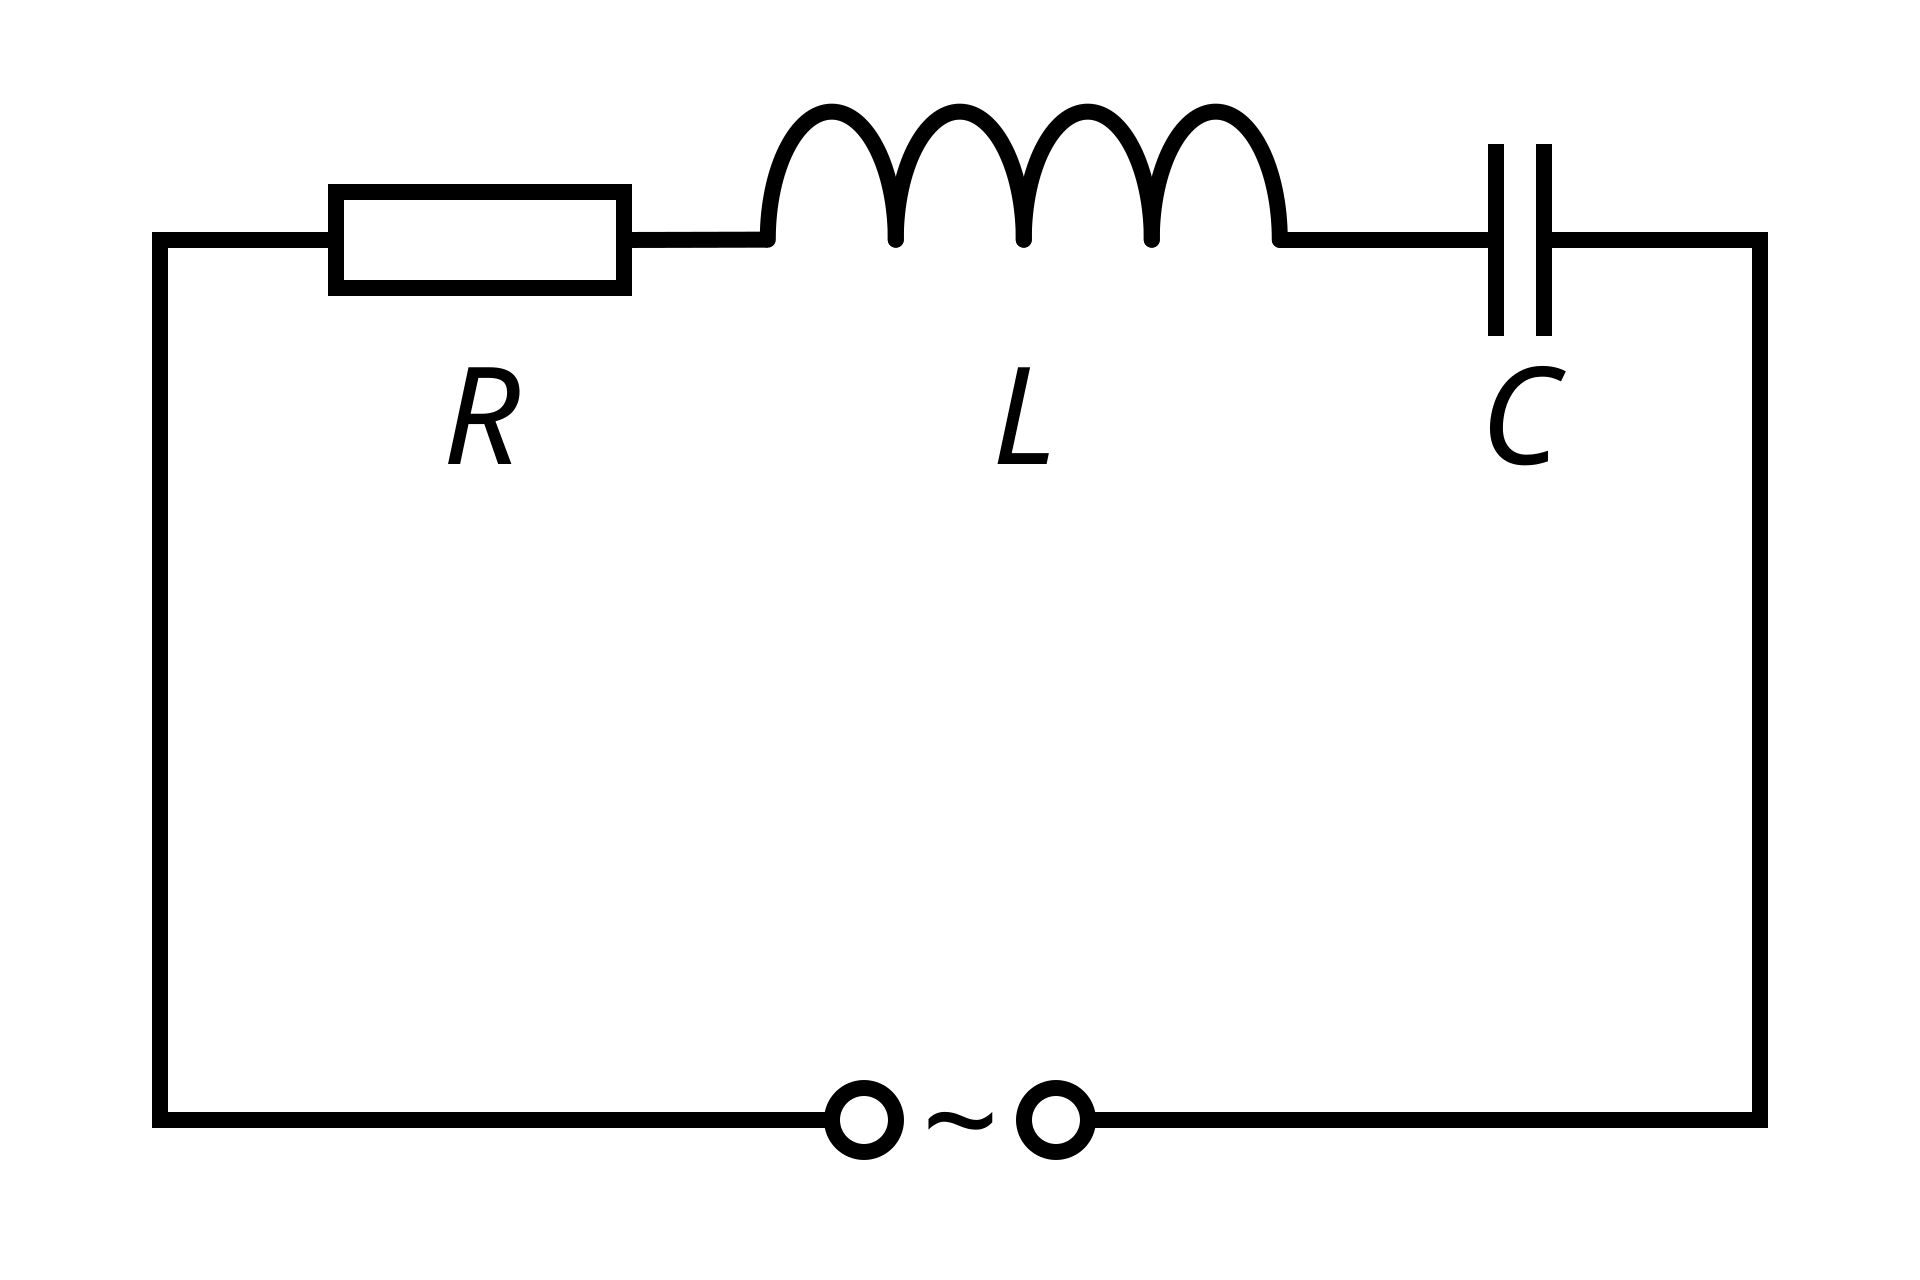
\includegraphics[width=0.5\textwidth]{Gedaempfter_Schwingkreis.png}
    \caption{Gedämpfter Schwingkreis\cite{gedaempfter_schwingkreis}}
    \label{fig:gedaempfter_schwingkreis}
\end{figure}
\subsection{Erzwungene Schwingungen}
Wird dem Schwingkreis eine zeitabhängig schwingende Spannung angelegt, schwingt der Schwingkreis mit der Frequenz der Spannung. In Abhängigkeit des Widerstands, der Kapazität und der Induktivität gibt es eine Frequenz, bei der ein Maximum an Energie in den Schwingkreis geführt werden kann. Es kommt zu einem Maximum der Stromamplitude bei dieser Resonanzfrequenz.

\subsection{Formeln}

%\section{Aufbau und Durchführung}
\section{Versuchsaufbau}
Für die folgenden Versuche werden folgende Bauteile auf unterschiedlichen Weisen miteinander verbunden und eingestellt. Es wird ein analoges Oszilloskop, in diesem Fall ein HAMEG HM-205-3(\ref{fig:oszilloskop}), ein Frequenzgenerator, hier ein HAMEG HM8030-4(\ref{fig:frequenzgenerator}), sowie ein Gerät, welches einen elektrischen Schwingkreis enthält benötigt. Letzteres Gerät setzt sich aus zwei festensowie einem variablen ohmschen Widerstand, einer Spule L und einem Kondensator C zusammen(\ref{fig:geraet2}). Weiterhin wird ein Tastkopf benötigt.
\begin{figure}[H]
    \centering

    \begin{subfigure}{0.45\textwidth}
        \centering
        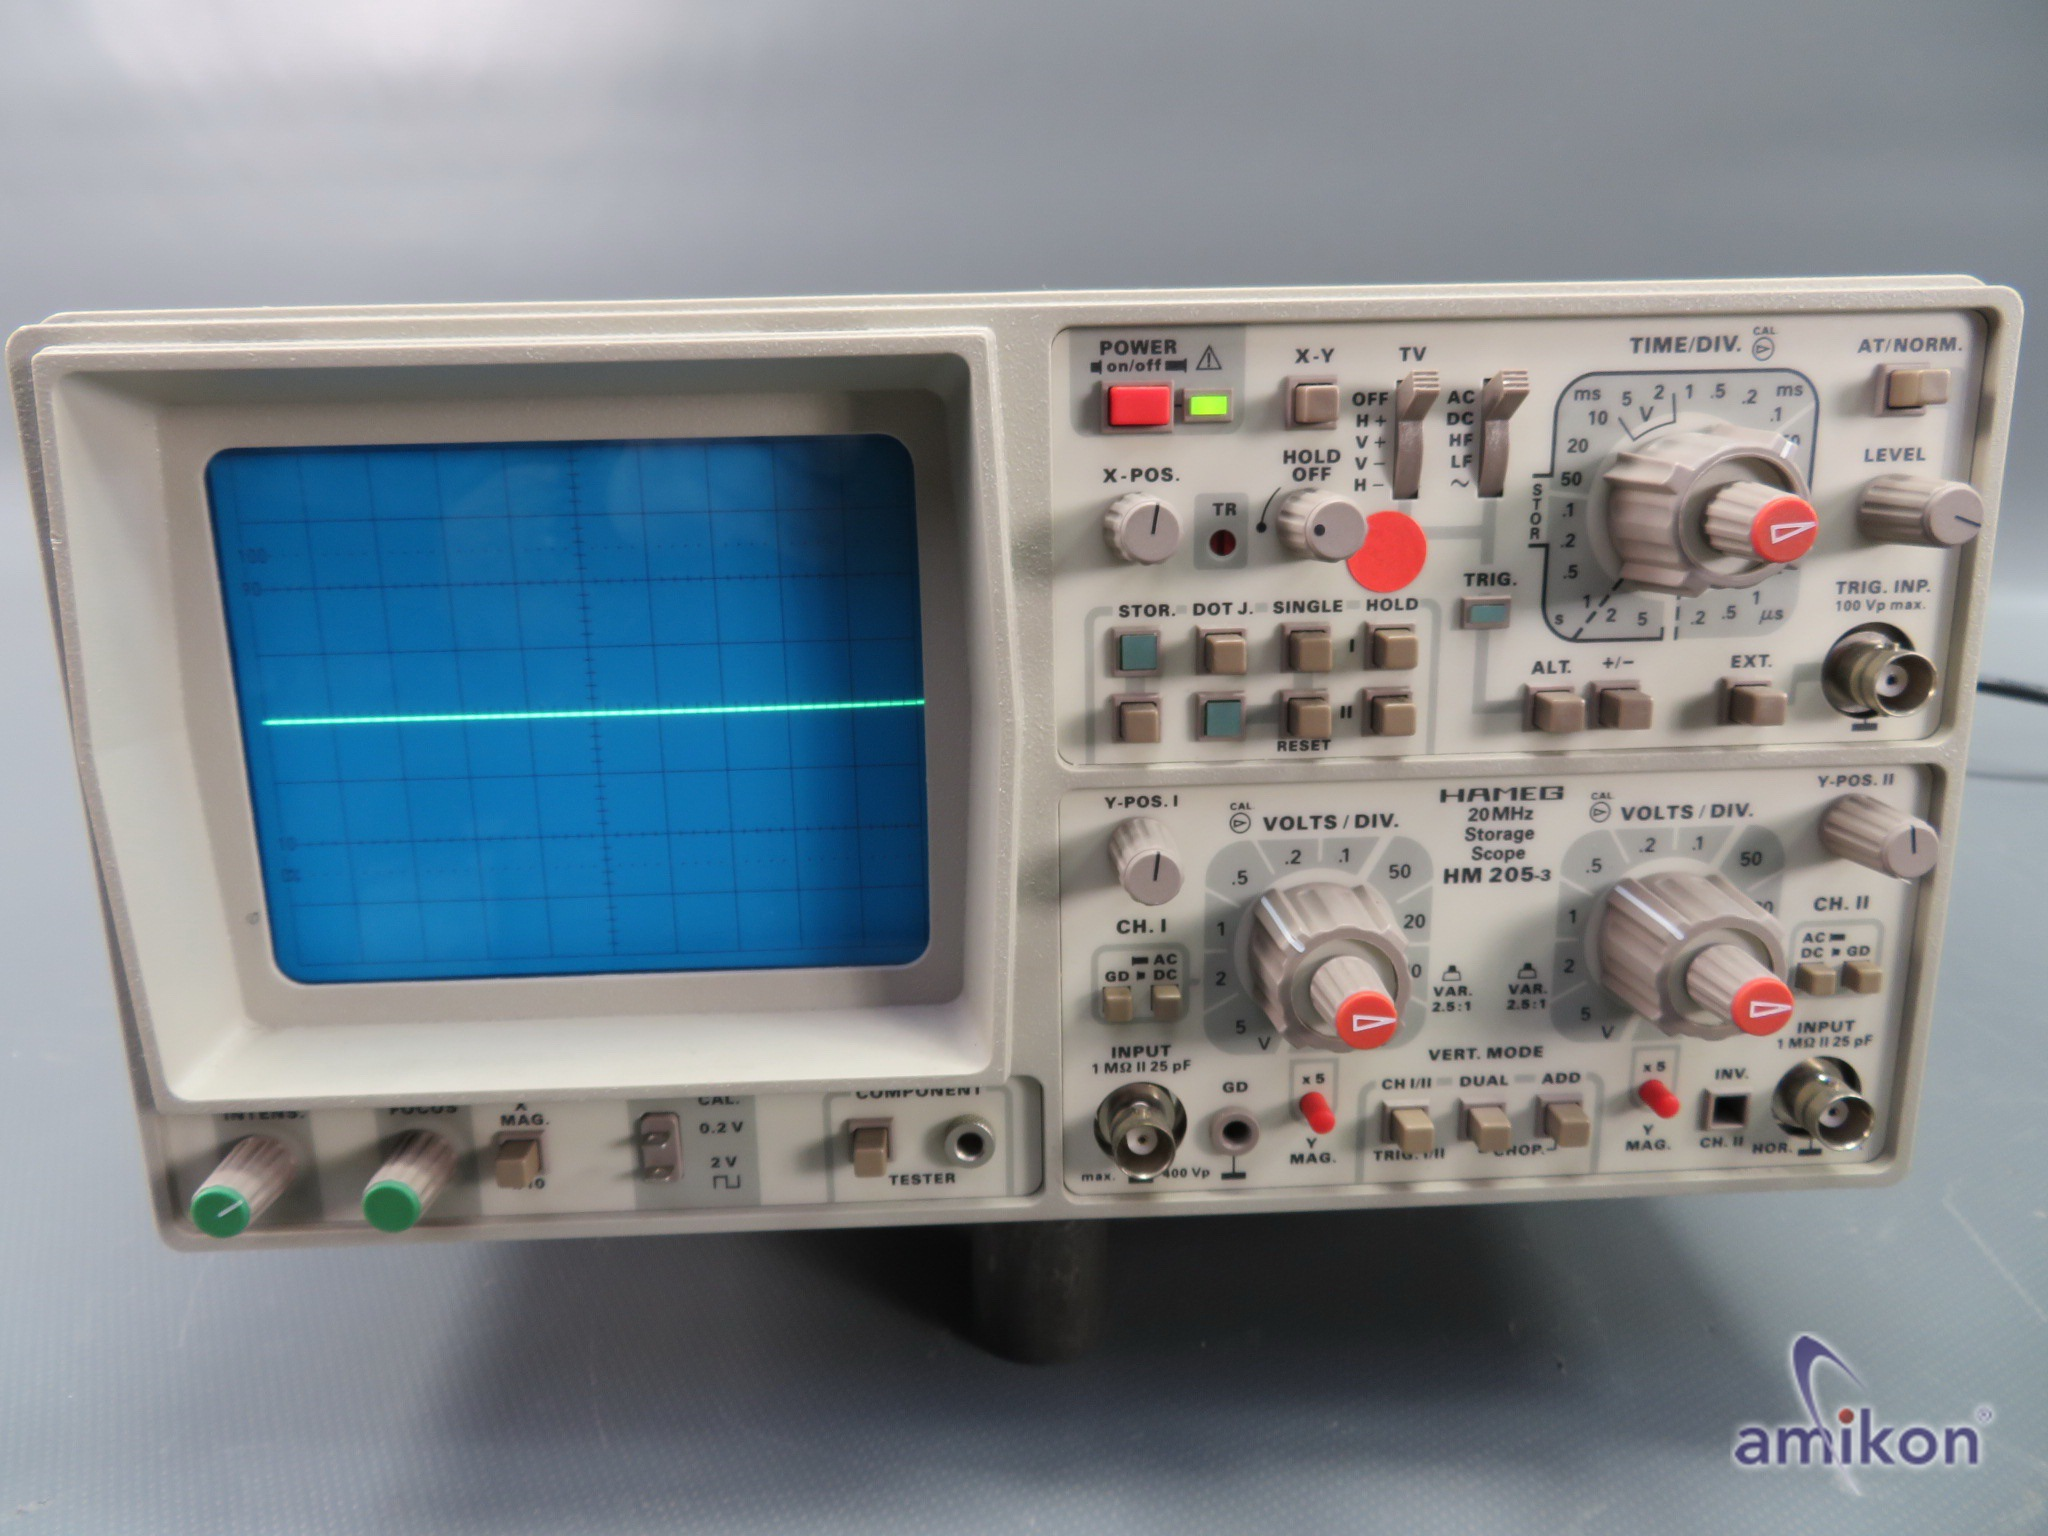
\includegraphics[width=\textwidth]{HAMEG-HM205-3.jpg}
        \caption{HAMEG Oszilloskop HM205-3\cite{Oszilloskop}}
        \label{fig:oszilloskop}
    \end{subfigure}
    \hfill
    \begin{subfigure}{0.45\textwidth}
        \centering
        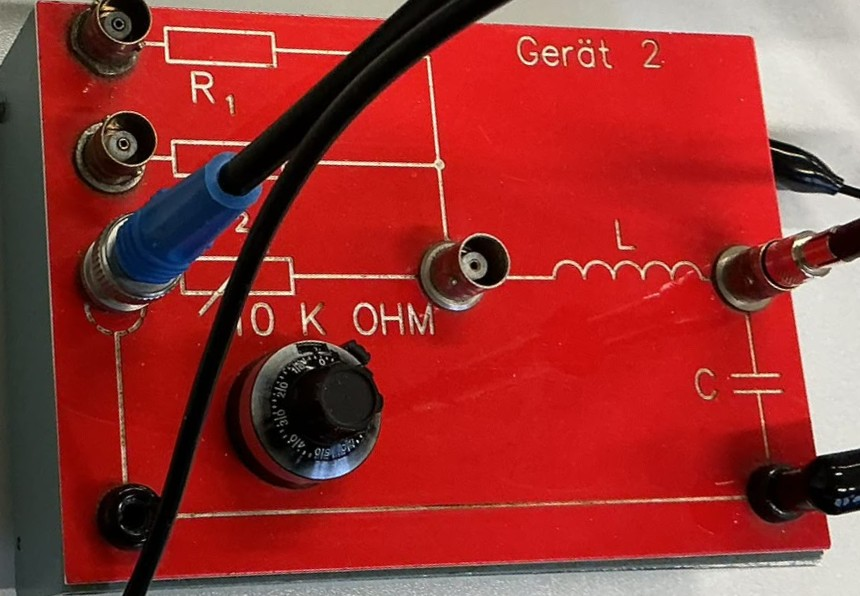
\includegraphics[width=\textwidth]{Geraet2.jpeg}
        \caption{Elektrischer Schwingkreis: Gerät 2 (eigene Aufnahme)}
        \label{fig:geraet2}
    \end{subfigure}
    \hfill
    \begin{subfigure}{0.45\textwidth}
        \centering
        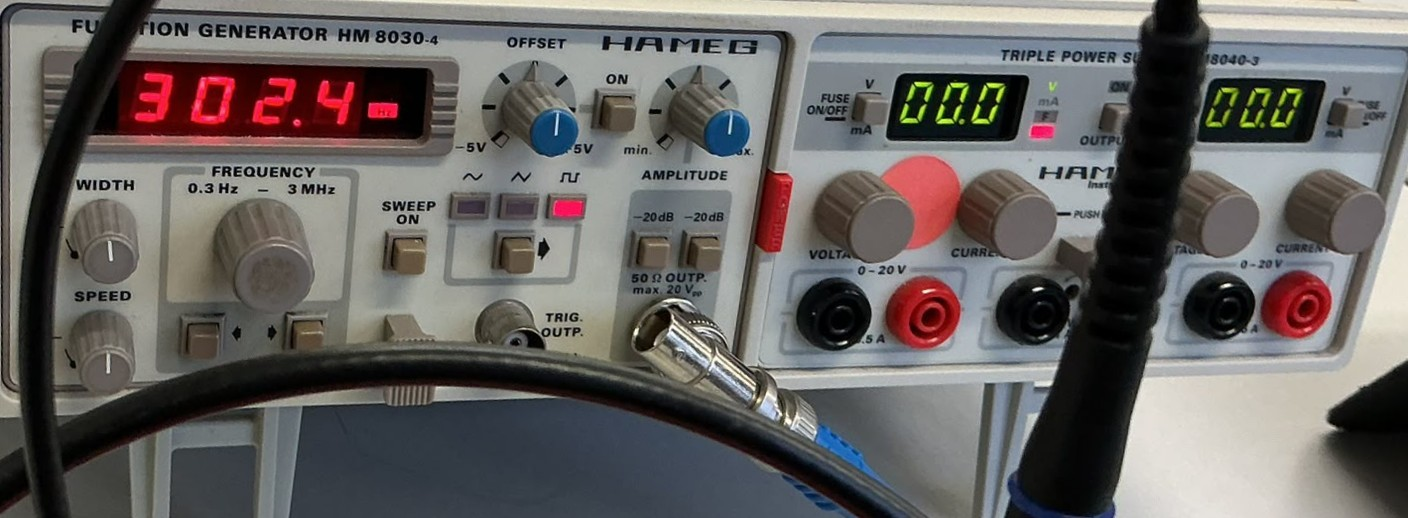
\includegraphics[width=\textwidth]{Frequenzgenerator.jpeg}
        \caption{Frequenzgenerator HAMEG HM8030-4 (eigene Aufnahme)}
        \label{fig:frequenzgenerator}
    \end{subfigure}
\end{figure}

\section{Durchführung}
Es werden in den folgenden Versuchen verschiedene Eigenschaften gedämpfter sowie erzwungener Schwingungen untersucht.
\subsection{Zeitabhängigkeit Amplitude}
Es wird zunächst die Zeitabhängigkeit der Schwingungsamplitude einer gedämpften Schwingung untersucht, um den kleineren der beiden Festwiderstände des Gerätes 2 zu bestimmen.
Dafür wird der Frequenzgenerator auf eine 302.4 Hz Sägezahnspannung eingestellt und an $R_1$ angeschlossen(\ref{fig:frequenzgenerator}). Der Tastkopf wird an den Abgriff nach der Spule $L$ und an den linken Input des Oszilloskops angeschlossen(\ref{fig:geraet2}). Für die Messung wird eine Einstellung des Oszilloskops von 0.2 V/DIV und 50$\mu$s/DIV gewählt und über die Peak-to-Peak Methode die Amplitude gemessen(\ref{fig:oszilloskop}).
\subsection{Aperiodischer Grenzfall}
In dieser Messung wird untersucht bei welchem Dämpfungswiderstand der Aperiodische Grenzfall eintritt. Dafür wird der vorherige Festwiderstand auf $R_1$ für den Regelbaren Widerstand ausgetauscht. Bei dem Oszilloskop wird die Einstellung 2$\mu$s/DIV gewählt(\ref{fig:oszilloskop}). Alle anderen Einstellungen werden nicht verändert. Der veränderbare Widerstand wird nun variiert, bis der aperiodische Grenzfall eintritt(\ref{fig:geraet2}).
Dies wird über zwei verschiedene Methoden bestimmt. Zunächst wird der Widerstand auf seinen Maximalwert eingestellt und dann langsam verringert, bis der aperiodische Grenzfall eintritt. Danach wird der Widerstand auf seinen Minimalwert eingestellt und langsam erhöht, bis der aperiodische Grenzfall eintritt. Die beiden Werte werden notiert und verglichen.
\subsection{Frequenzabhängigkeit Spannung und Phase}
Um die Frequenzabhängigkeit der Kondensator- und Erregerspannung sowie ihrem Phasenunterschied zu untersuchen, wird anstelle des einstellbaren Widerstandes der größere feste Widerstand $R_2$ eingesetzt(\ref{fig:geraet2}). Weiterhin wird der Trigger Output des Frequenzgenerators mit dem Trigger Input des Oszilloskops verbunden. Die Spannung des Frequenzgenerators wird außerdem direkt an den rechten Input des Oszilloskops angeschlossen und als Sinusspannung gewählt(\ref{fig:frequenzgenerator}).
Das Oszilloskop wird auf beiden Seiten auf 0.5 V/DIV und insgesamt auf 10$\mu$s/DIV eingestellt. Über den Dual Knopf werden beide Spannungen angezeigt(\ref{fig:oszilloskop}). 
Zunächst wird die Resonanzfrequenz bestimmt, indem die Frequenz des Frequenzgenerators variiert wird, bis die maximale Kondensatorspannung erreicht wird. Die Spannungen des Kondensators und des Erregers werden über die Peak-to-Peak Methode gemessen und notiert. Es wird der Phasenunterschied der beiden Spannungen über bestimmung des Zeitunterschieds zwischen den Peaks der Spannungen sowie der Periodendauer der Kondensatorspannung berechnet. Dieser Vorgang wird nun in zehn mal in 0.5 kHz Schritten jeweils nach unten und oben wiederholt, sowie bei 10 kHz, bei 20 kHz und bei 50 kHz(\ref{fig:frequenzgenerator}).
\section{Auswertung und Diskussion}
In den Versuchen hatten die verwendeten Bauteile folgende Werte, welche im folgenden
für die Auswertung verwendet werden:
\begin{itemize}
    \item Widerstand 1: $R_1 = 48,1 \pm 0,1 \mathrm{ohm}$
    \item Widerstand 2: $R_2 =509,5 \pm 0,5 \mathrm{ohm}$
    \item Kondensator: $C = 2,089 \pm 0,006 \mathrm{nF}$
    \item Spule: $L = 10,11 \pm 0,03 \mathrm{mH}$
\end{itemize}
\subsection{Zeitabhängikeit der Amplitude}
Um die Zeitabhängigkeit der Amplitude zu bestimmen, wurde die Spannung $U$ in Abhängigkeit der Zeit $t$ gemessen. 
Die Messwerte sind in Tabelle 1 dargestellt. 
\begin{table}[H]
    \centering
    \begin{tblr}{c c c}
    \toprule
    $Messung$ & $Spannung$  U in V & Zeit $\delta t$ in $\mu$s \\
    \midrule
    $T_0$ & 0.62 & 20 \\
    $T_1$ & 0.57 & 30 \\
    $T_2$ & 0.53 & 50 \\
    $T_3$ & 0.48 & 60 \\
    $T_4$ & 0.43 & 75 \\
    $T_5$ & 0.40 & 90 \\
    $T_6$ & 0.36 & 105 \\
    $T_7$ & 0.33 & 120 \\
    $T_8$ & 0.30 & 135 \\
    $T_9$ & 0.27 & 150 \\
    $T_{10}$ & 0.25 & 165 \\
    $T_{11}$ & 0.23 & 180 \\
    $T_{12}$ & 0.21 & 195 \\
    $T_{13}$ & 0.20 & 210 \\
    $T_{14}$ & 0.18 & 225 \\
    $T_{15}$ & 0.16 & 240 \\
    \bottomrule 
    \end{tblr}
    \caption{Messreihe zur Zeitabhängigkeit der Amplitude}
\end{table}
\noindent
Die Zeit wurde in delta t gemessen, da die Zeit zwischen den einzelnen Peaks der Spannung gemessen wurde.
Die Spannung wurde über die Peak-to-Peak Methode bestimmt, und dann durch zwei geteilt, um die Amplitude zu erhalten.
Aus den Messwerten wurde ein Fit der Form $U(t) = U_0 \cdot e^{-\frac{R}{2L}t}$ durchgeführt, um den Widerstand R zu bestimmen.
Die Messwerte und der Fit sind in Abbildung 3 dargestellt.
\begin{figure}[H]
    \centering
    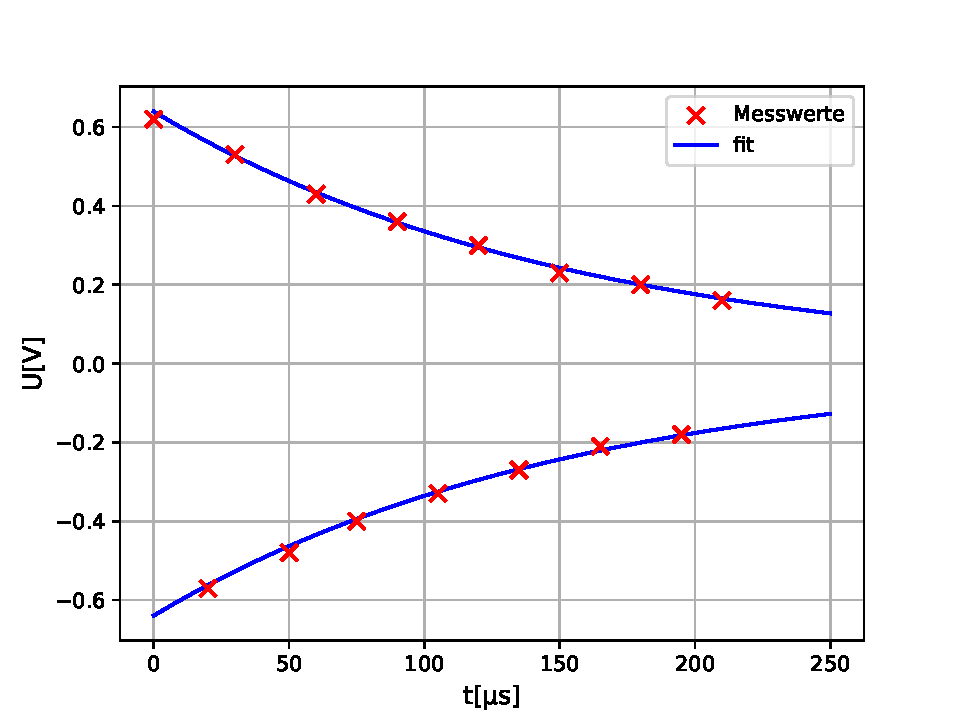
\includegraphics[width=0.8\textwidth]{v354/Exp_Abfall.pdf}
    \caption{Messwerte und Fit der Zeitabhängigkeit der Amplitude}
    \label{fig:exp_abfall}
\end{figure}
\noindent
Der Fit wurde in der Form $f(x) = a \cdot e^{b \cdot x}$ durchgeführt, wobei $a$ und $b$ die Fitparameter sind.
Aus dem Fit wurde der Wiederstand R bestimmt(\ref{fig:exp_abfall}). Der Fit ergab einen Wert von $b = -6449.56 \pm 102,52 \mathrm{Hz}$. Daraus ergibt sich ein Widerstand von:
\begin{equation}
    R_{\text{Fit}} = 2 \cdot L \cdot b \cdot (-1) = 130,39 \mathrm{\Omega}
\end{equation}
Die Ungenauigkeit des Widerstands wurde über die Fehlerfortpflanzung bestimmt. Die Fehlerfortpflanzung ergibt sich aus der Formel:
\begin{equation}
    \Delta R = \sqrt{(\frac{\partial R}{\partial L} \cdot \Delta L)^2 + (\frac{\partial R}{\partial b} \cdot \Delta b)^2}
\end{equation}
Damit ergibt sich eine folgende Ungenauigkeit des Widerstands:
\begin{gather}
    \Delta R = 2 \cdot \sqrt{(b \cdot \Delta L)^2 + (L \cdot \Delta b)^2} = 2 \\
    \sqrt{(6449,56 \cdot 0,03)^2 +(10,11 \cdot 102,52)^2} = 2,08 \mathrm{\Omega}\\
    R_{\text{Fit}} = 130,39 \pm 2,08 \mathrm{\Omega}
\end{gather}

\subsection{Aperiodischer Grenzfall}
Der Widerstand, der für den Aperiodischen Grenzfall benötigt wird, lässt sich mit folgender Formel bestimmen:
\begin{equation}
    R_{\text{Theorie}} = 2 \cdot \sqrt{\frac{L}{C}}
\end{equation}
Damit ergibt sich ein Widerstand von:
\begin{equation}
    R_{\text{Theorie}} = 2 \cdot \sqrt{\frac{10,11 \cdot 10^{-3}}{2,089 \cdot 10^{-6}}} = 4399,83 \mathrm{\Omega}
\end{equation}
Der Aperiodische Grenzfall wurde über ein vestellbaren Widerstand bestimmt, der zwischen 1 und 10000 Ohm einstellbar ist.
 Der Widerstand wurde zunächst auf seinen Maximalwert eingestellt und dann langsam verringert, bis der Aperiodische Grenzfall eintrat. 
 Danach wurde der Widerstand auf seinen Minimalwert eingestellt und langsam erhöht, bis der Aperiodische Grenzfall eintrat. 
Der Aperiodische Grenzfall trat beim ersten Versuch bei einem Widerstand von $R_{\text{exp1}} \approx 3200 \mathrm{\Omega}$ ein.
Beim Zweiten Versuch trat der Aperiodische Grenzfall bei einem Widerstand von $R_{\text{exp2}} \approx 3160 \mathrm{\Omega}$ ein.
\subsection{Frequenzabhängigkeit der Kondensatorspannung und Phase}
Um die Frequenzabhängigkeit der Kondensatorspannung und der Phase zu bestimmen, 
wurde die Spannung des Kondensators $U_C$ und die Spannung des Erregers $U_{Err}$ in Abhängigkeit der Frequenz $f$ gemessen, siehe Tabelle 2.
\begin{table}[H]
    \centering
    \caption{Frequenzabhängigkeit der Kondensatorspannung und Phase}
    \begin{tblr}{c c c c}
    \toprule
    Frequenz in $kHz$ & $U_C$ in V & $U_{Err}$ in V & Verschiebung \\
    \midrule
    10.0 & 1.05 & 0.8 & 0.00 \\
    20.0 & 1.25 & 0.8 & 0.00 \\
    27.9 & 2.05 & 0.8 & 0.3 \\
    28.4 & 2.15 & 0.8 & 0.3 \\
    28.9 & 2.25 & 0.8 & 0.3 \\
    29.4 & 2.35 & 0.8 & 0.4 \\
    29.9 & 2.45 & 0.8 & 0.4 \\
    30.4 & 2.55 & 0.8 & 0.5 \\
    30.9 & 2.65 & 0.8 & 0.5 \\
    31.4 & 2.75 & 0.8 & 0.6 \\
    31.9 & 2.85 & 0.8 & 0.6 \\
    32.4 & 2.85 & 0.8 & 0.6 \\
    32.9 & 2.85 & 0.8 & 0.7 \\
    33.4 & 2.85 & 0.8 & 0.7 \\
    33.9 & 2.80 & 0.8 & 0.8\\
    34.4 & 2.70 & 0.8 & 0.8 \\
    34.9 & 2.55 & 0.8 & 0.8 \\
    35.4 & 2.45 & 0.8 & 0.9 \\
    35.9 & 2.35 & 0.8 & 0.9 \\
    36.4 & 2.15 & 0.8 & 1 \\
    36.9 & 2.10 & 0.8 & 1\\
    37.4 & 1.95 & 0.8 & 1 \\
    37.9 & 1.85 & 0.8 & 1 \\
    50.0 & 0.65 & 0.8 & 0.9 \\
    \bottomrule
    \end{tblr}
\end{table}
Damit ergibt sich die Resonanzfrequnez aus der Messung bei $f_{\text{res}} = 32,9 \mathrm{kHz}$.
Die Theoriewerte für die Resonanzfrequenz und die Güte des Schwingkreises lassen sich über folgende Formeln bestimmen:
\begin{equation}
    f_{\text{res, Theorie}} = \frac{1}{2 \pi \sqrt{L \cdot C}} = 34,7 \mathrm{kHz}
\end{equation}
Und die Kondensatorspannung in abhängigkeit der Frequenz lässt sich über folgende Formel bestimmen:
\begin{equation}
    U_C(f) = \frac{U_0}{\sqrt{(1 - (2 \pi f)^2 L C)^2 + (2 \pi f R C)^2}}
\end{equation}
Den Plot der Kondensatorspannung und der Phase in Abhängigkeit der Frequenz ist in Abbildung 4 dargestellt.
\begin{figure}[H]
    \centering
    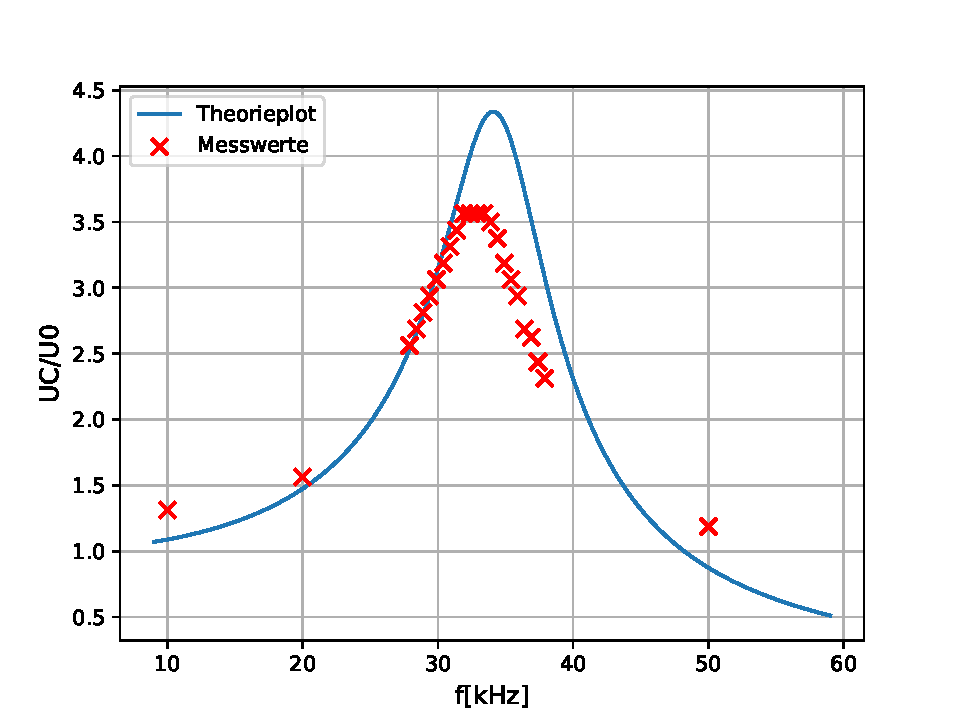
\includegraphics[width=0.8\textwidth]{v354/Spannungsamplitude.pdf}
    \caption{Kondensatorspannung in Abhängigkeit der Frequenz}
    \label{fig:amp}
\end{figure}
Die Phasenverschiebung lässt sich über folgende Formel bestimmen:
\begin{equation}
    \phi(f) = \arctan{\Bigl(\frac{-2 \pi f R C}{1 - (2 \pi f)^2 L C}\Bigr)}
\end{equation}
Die aus den Messwerten bestimmte Phasenverschiebung ist in abhängigkeit der Frequenz in Abbildung 5 dargestellt.
\begin{figure}[H]
    \centering
    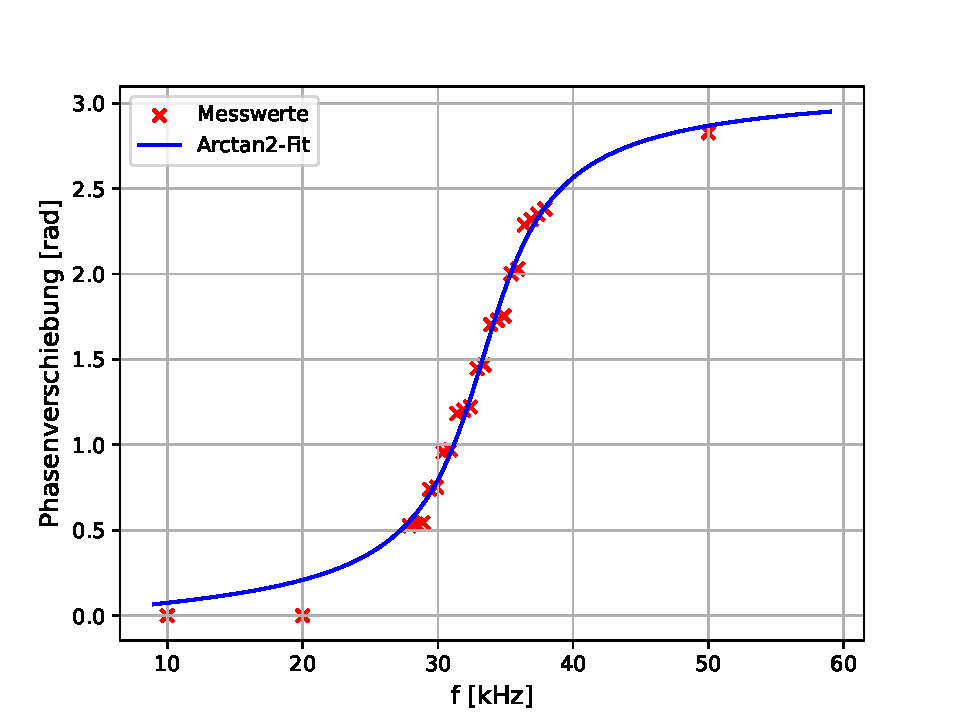
\includegraphics[width=0.8\textwidth]{v354/Arctan2.pdf}
    \caption{Phasenverschiebung in Abhängigkeit der Frequenz}
    \label{fig:phase}
\end{figure}
\subsection{Güte des Schwingkreises}

4 Wege Güte zu errechnen
Theoriewert Resonanzbreite aus amp.plot%1/sqrt(2)
Hochpunkt aus amp.plot
resonanzbreite aus phasen.plot (45,90,135 grad)
\printbibliography{}
\section{Code}
\inputminted{python3}{v354/v354.py}
\end{document}